\documentclass[11pt]{article}

\usepackage{float}
\usepackage{hyperref}
\usepackage{fullpage}
\usepackage{verbatim}
\usepackage{moreverb}
\usepackage{graphicx}
\usepackage{minted}
\let\verbatiminput=\verbatimtabinput
\def\verbatimtabsize{4\relax}

\begin{document}
\title{EECS 151/251A FPGA Lab\\
Lab 3: Useful Digital Circuits for Basic Signal Processing, Finite State Machines, and Synchronous Resets}

\author{Prof. Borivoje Nikolic \\
TA: Vighnesh Iyer \\Department of Electrical Engineering and Computer Sciences\\
College of Engineering, University of California, Berkeley}
\date{}
\maketitle

\section{Before You Start This Lab}

Before you proceed with the contents of this lab, we suggest that you look through three documents that will help you better understand some concepts we will be covering.

\begin{enumerate}
	\item \textbf{labs\_fa16/docs/Verilog/verilog\_fsm.pdf}
	
	Goes over concepts of FSM in Verilog. Provides an example of  implementing FSM's in Verilog and pitfalls to watch out for.
	
	\item \url{http://www.labbookpages.co.uk/electronics/debounce.html}
	
	Read the "What is Switch Bounce" section to get idea of why we need a debouncer circuit. Read the "Digital Switch Debouncing" section to get a general overview of the circuit, its parts, and their purposes. You may want to pay attention to the purpose of the synchronizer as meta-stability is something you will go over in class.
	
	\item \url{http://www.xilinx.com/products/boards/s3estarter/files/s3esk_rotary_encoder_interface.pdf}
	
	Read slide 5 (Rotary Encoder and Signals) to get an idea of how the encoder works and the signal it generates. You can read the next few pages to get a better idea of how to use the signals. You will be implementing the circuit described in these slides in this lab.

\end{enumerate}

In the first couple sections of this lab, we will be revisiting the circuit you did in lab 2 and confirming their functionality with music generated by the updated Python scripts. Then we will be going over some new circuits that you will be using in future assignments.

\subsection{Helpful Hint: Synthesis Warnings and Errors}
At various times in this lab, things will just not work on the FPGA or in simulation. To help with debugging, you can run \verb|make synth| in the \verb|lab3/| folder. This will just run \verb|xst| which will only take a few seconds. Then you should run \verb|make report|. In the window that opened, click on \verb|Synthesis Messages| on the left under \verb|Errors and Warnings|. Any synthesis warnings you see here are a possible alert to some issue in your circuit. If you don't understand a warning, ask a TA; it almost always reveals some issue in your RTL.

% Let's not even mention this
% If your reports indicate there are no issues but you still have problems, please make sure that it is working in simulation. There is one case related to how memory is generated where you will likely get different results between simulation and actual FPGA behavior but we do not expect it to occur in this lab. This is an issue we will discuss in later in the lab. 

You should keep the depth and width of the ROM consistent throughout the lab. We recommend generating a ROM that's 24 bits wide and 4096 addresses deep (12-bit addresses).
\section{Lab Overview}

In this lab, we will begin by taking your \verb|tone_generator| and \verb|music_streamer| design from Lab 2 and feeding it some music. We will learn about circuits to take the signals generated by the buttons and rotary encoder on the ML505 board and convert them into a digital signal we can use in our FPGA design. You will be using the LED's to confirm they are working correctly. We will discuss how to use synchronous resets to set an initial state of your circuits.\\

Run \verb|git pull| in your \textbf{git cloned} \verb|labs_fa16| directory to \textbf{fetch the latest skeleton files for this lab.}

\section{Overview of Your Tone\_generator and Music\_streamer}

\begin{center}
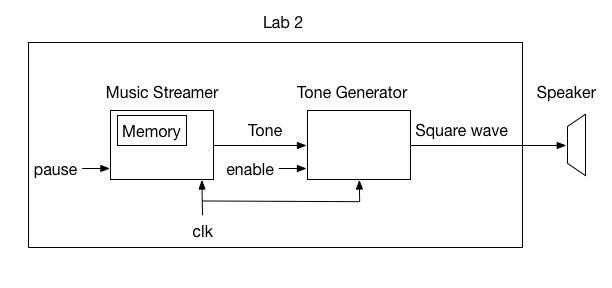
\includegraphics[height=5cm]{images/lab2_fig1.png}
\end{center}

We included this diagram so you can review the circuit you made in lab 2. There are two main modules that you created: \verb|tone_generator| and \verb|music_streamer|. \\

Your \verb|tone_generator| should take an input signal representing the tone or frequency you want to play and output a square wave that goes to the piezo speaker. It has an enable signal that allows you to disable the output, and this enable signal should be hooked up to one of the DIP switches.  \\

Your \verb|music_streamer| is responsible for providing the input signal to your \verb|tone_generator| so it knows what frequency to play. Inside this generator is the memory (ROM), that holds the frequencies you want to play. Your music generator will output one tone for a certain amount of time (1/5 of a second for lab 2) before incrementing the ROM's address input. Your \verb|music_streamer| will keep incrementing its address until it reaches the end of the ROM after which it should reset back to the first address, and loop through the ROM again.

\section{ROM and music\_streamer Modifications}
Copy your \verb|music_streamer| and \verb|tone_generator| implementations from lab 2 into \verb|lab3/src/music_streamer.v| and \verb|lab3/src/tone_generator.v| respectively. 

\subsection{Generating a ROM}
Run the following scripts in the \verb|lab3/| directory to generate a Verilog ROM from sheet music.\\

First, use the \verb|musicxml_parser.py| script to convert sheet music (in the form of a MusicXML file) into the contents of the ROM.

\begin{minted}[frame=single]{bash}
python scripts/musicxml_parser.py musicxml/Row_Row_Row_Your_Boat.xml music.txt
\end{minted}

You will now have a \verb|music.txt| file in the \verb|lab3/| directory with the ROM's contents. Now we use \verb|rom_generator.py| to create a ROM using this file.

\begin{minted}[frame=single]{bash}
python scripts/rom_generator.py src/rom.v music.txt 4096 24
\end{minted}

You will now have a \verb|rom.v| file in \verb|lab3/src|. Take a look at this file. The ROM is 4096 entries deep and 24 bits wide with a 12-bit address input. 

You can use any sheet music you want that's available in MusicXML. This website \url{https://musescore.com/} has a lot of good quality sheet music that you can download and play on the FPGA!

\subsection{music\_streamer Modifications}

Make the following changes to the \verb|music_streamer|:

\begin{enumerate}
	\item Modify your code to use a 12-bit ROM address
	
	\item Output the ROM address through the \verb|rom_address| output. The most significant 8 bits of your ROM address will show up on the 8 GPIO LEDs.
	
	\item Modify the amount of time each tone in the ROM will play to be $\frac{1}{25}$th of a second from $\frac{1}{5}$th of a second in lab 2.
	
	\item There is a new output from the ROM called \verb|last_address|. It contains the last address of the ROM that should be played. After you traverse the ROM and get to the last address, you should loop back to address 0.
\end{enumerate}

You shouldn't need to make any changes to your \verb|tone_generator| from lab 2.

\section{Playing Music}
Go through the FPGA tool flow by running \verb|make|. Check \verb|make report| to see if there are any unexpected synthesis warnings; ask the TA if you need clarification. Run \verb|make impact| and you should be able to hear 'Row Row Row Your Boat' playing through the piezo speaker. \\

{\footnotesize * One issue you probably won't run into but should be aware of is that the tools will infer distributed memory on SLICEMs as long as our ROM module is small enough. If the ROM we specify is too big, then the tools will infer block RAMs instead. Block RAMs are synchronous memories which our \verb|music_streamer| isn't designed to use; we will learn more about synchronous RAM in the next lab.}

\section{Synchronizer, Debouncer, and Rotary Encoder}

\begin{center}
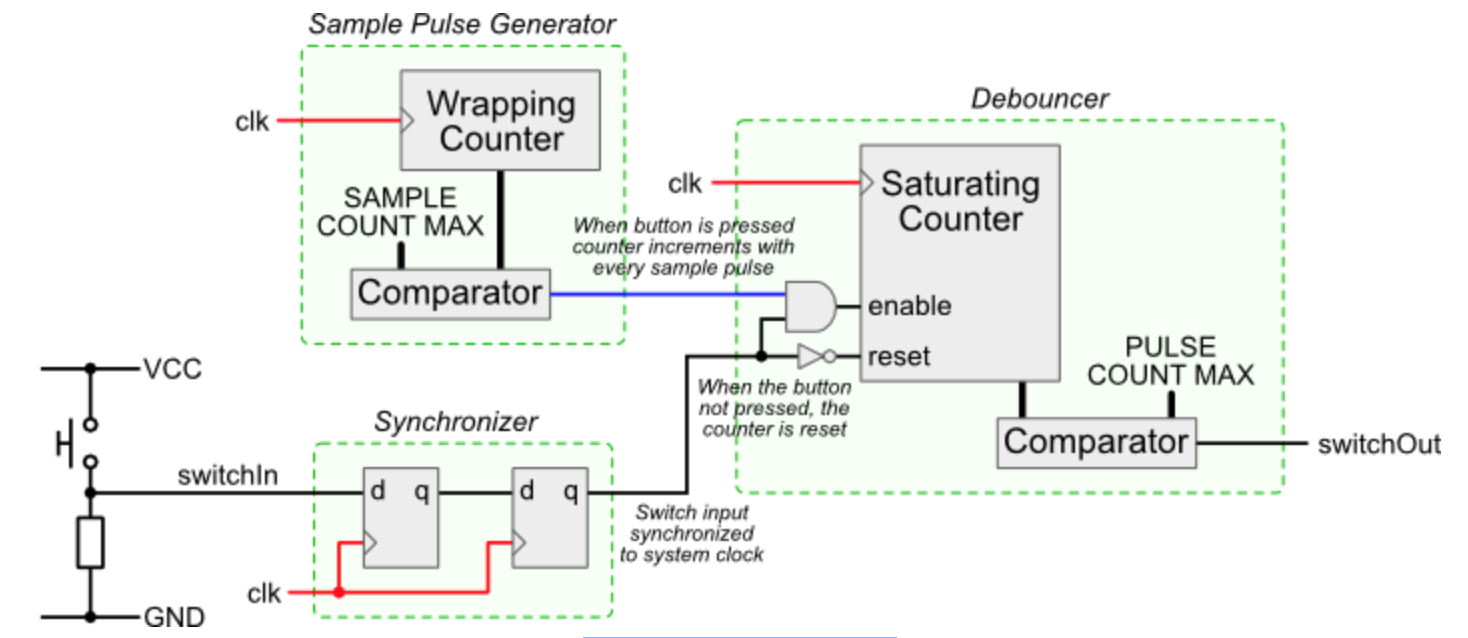
\includegraphics[height=5cm]{images/lab2_fig2.png}
\end{center}

Recall this graphic from the prelab debouncer reading. It is an overview of the debouncer circuit which includes the synchronizer circuit.

\subsection{Synchronizer}
In RTL, digital signals can be interpreted as 0's and 1's. However, in reality these correspond to low and high voltages and there are other states that can occur. In the lab we have to be concerned about the metastable state.

\begin{center}
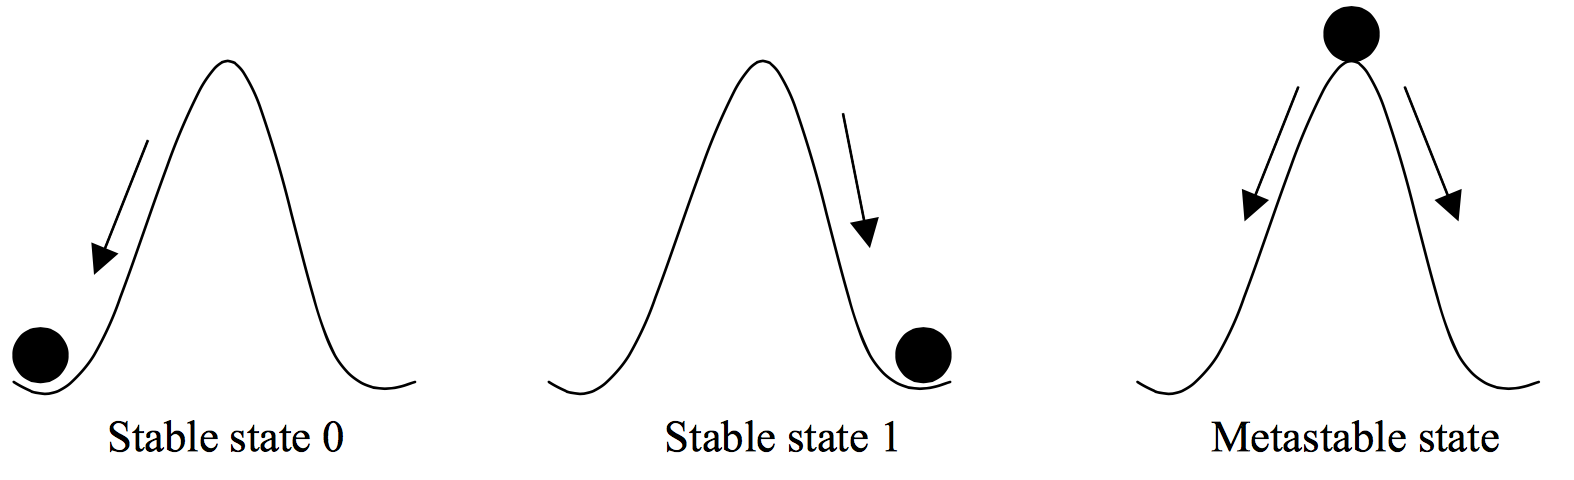
\includegraphics[height=3cm]{images/lab2_fig3.png}
\end{center}

Normally, when there are no timing issues, we only have to worry about the high and low states. However, if there are timing issues, we can run into metastability where a net is basically stuck between the two states. This is an oversimplification but what you ultimately need to know is that metastability is generally undesirable and we want a circuit to get rid of it. \\

This synchronizer circuit we want you to implement for this lab is relatively simple. For synchronizing one bit, it is a pair a flip-flops connected serially. This circuit synchronizes an asynchronous signal (not related to any clock) coming into the FPGA. We will be using our synchronizer circuit to bring any off-FPGA signals into the clock domain of our FPGA design.\\

Edit the \verb|lab3/src/synchronizer.v| file to implement the two flip-flop synchronizer. This module is parameterized by a \verb|width| parameter which indicates the number of one-bit signals to synchronize.

\subsubsection{Testing}
As a rudimentary test of your synchronizer, we have provided a file called \verb|lab3/src/synchronizer_fpga_test.v| which will synchronize various button press signals and send them to the GPIO LEDs. Execute the following commands:

\begin{minted}[frame=single]{bash}
make TOP=synchronizer_fpga_test
make TOP=synchronizer_fpga_test report
make TOP=synchronizer_fpga_test impact
\end{minted} 

We are changing the default value of \verb|TOP| that the \verb|Makefile| uses, to point to \verb|synchronizer_fpga_test| as the top level module rather than \verb|ml505top|. This allows us to build and impact different top level modules in the same folder. Keep in mind that each top level module needs a UCF file with the same name defining its I/O.

Take a look at this test module and try it out on the board. Pressing the various buttons should light up the respective LED. \\

You will notice that when pressing certain buttons, the LED flickers on and off before setting at on. This can create issues in our digital logic if we just assume that a low to high logic level transition constitutes a button press, since we will get erroneous presses. We use a debouncer to fix this issue.

\subsection{Debouncer}

For this lab, the debouncer circuit will take a button's digital input and output a single pulse indicating a single button press. The reason we need a somewhat involved circuit for this is shown in the figure below.

\begin{center}
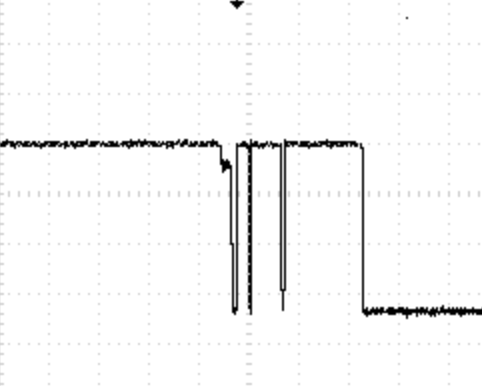
\includegraphics[height=5cm]{images/lab2_fig4.png}
\end{center}

When we press the button, we don't get a perfect stable signal. Instead the button signal has a mechanical 'bounce'. A debouncer turns this waveform, which shows a single button press, into a single pulse that our circuit can use.

Take a look at \verb|lab3/src/debouncer.v|. This is a parameterized debouncer which can debounce \verb|width| signals at a time. Your debouncer receives a vector of synchronized 1-bit signals and it outputs a debounced version of those signals. The other parameters reference the constants used in the circuit from the prelab reading.

The debouncer consists of:

\begin{enumerate}
	\item \textbf{Sample Pulse Generator} - Tells our main debouncer counter when to sample the input signal. It should output a 1, every \verb|sampling_pulse_period| clock cycles. By default \verb|sampling_pulse_period| is set to 25000.
	
	\item \textbf{Saturating Counter} - This is a counter that counts up to \verb|saturating_counter_max|. Every time the sample pulse generator tells the saturating counter to sample the input signal, it should either count up by 1 if the input signal is high, or it should reset to zero if the input signal is low. When the saturating counter reaches the value of \verb|saturating_counter_max|, by default set to 120, it should output a pulse that's one clock period wide. (i.e. the saturating counter should reset to zero the cycle after the counter reaches \verb|saturating_counter_max|. This isn't shown in the circuit diagram.)
\end{enumerate}

You will likely need to use 2D regs in Verilog to implement a saturating counter for each input signal to debounce. You will also likely need to use generate-for. You can use the same sample pulse generator for all input signals.

As an example:

\begin{minted}{verilog}
reg [7:0] arr [0:3]; // 4 x 8 bit array
arr[0]; // First byte from arr (8 bits)
arr[1][2]; // Third bit of 2nd byte from arr (1 bit)

genvar i;
generate
	for (i = 0; i < width; i = i + 1):LOOP_NAME begin
		// Insert Verilog here
		always @ (posedge clk) begin
			// Stuff
		end
	end
endgenerate
\end{minted}

\subsubsection{Testing in Simulation}
There is no staff created testbench for this module, but you are welcome to create your own. Instantiate your debouncer and synchronizer module and feed it a simulated button press. First start the button off low, then after x ns make it high and oscillate it a bit before settling at high in your initial block. Run your simulation for a second or so and see how your debouncer module behaves. You will have to write your own testbench file and your own .do file to be placed in \verb|lab3/sim/tests| for this testbench.

\subsubsection{Testing on the FPGA}
We have created a top level module called \verb|debouncer_fpga_test| that will create a 8-bit register and will use button presses to add and subtract from it. Pressing any button will cause the counter to increment and the LEDs will show the current value of the counter. Pressing the South compass button however, will cause the counter to decrement. 

\begin{minted}[frame=single]{bash}
make TOP=debouncer_fpga_test
make TOP=debouncer_fpga_test report
make TOP=debouncer_fpga_test impact
\end{minted} 

Make sure that your report gives you \textbf{zero warnings for synthesis.} You must fix any and all warnings before your debouncer will work well on the FPGA.\\

\textbf{Show the TA the debouncer working before moving on. It is critical that your debouncer works properly.}

You will discover when playing with your debouncer that the buttons have a way that they like being pressed to minimize bounce; get a good feel for them. You can try holding down a button to see how your debouncer will only output pulses at a regular interval. You can try changing the debouncer parameters to see how they affect the debouncer's performance.

\subsection{Rotary Encoder}

The rotary encoder consists of a circuit that has two switches that go high as you rotate the wheel. Recall this waveform from the prelab reading.

\begin{center}
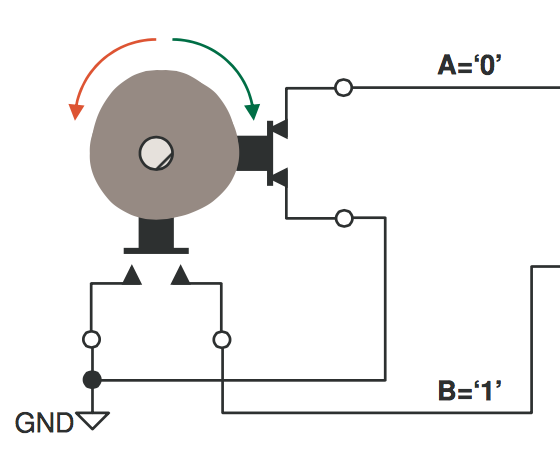
\includegraphics[height=5cm]{images/lab2_fig5.png}
\end{center}

Our main concern is finding out which direction the wheel turned. The following oscilloscope waveform from the prelab reading illustrates how we will do so. 

\begin{center}
	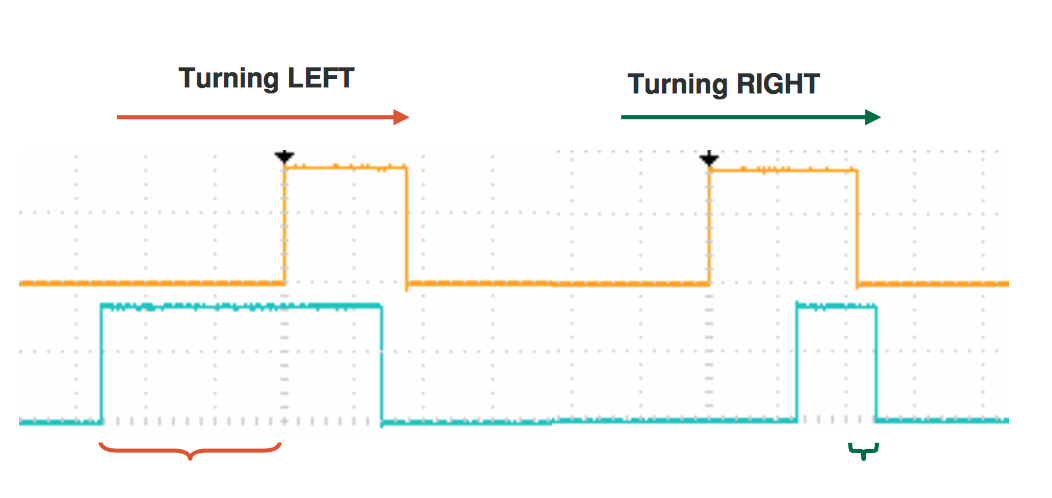
\includegraphics[height=5cm]{images/lab2_fig6.png}
\end{center}

If the pulse from A (top wave - orange) happens before the pulse from B (bottom wave - blue), it indicates that a the wheel has been turned a certain way. If the wheel is spun in the opposite direction then B's pulse will occur before A. We will take advantage of the fact that we can examine the logic level of wave B at the rising edge of wave A to determine direction of wheel movement.

Open up \verb|lab3/src/rotary_decoder.v|. This module takes the synchronized A and B signals, and a clock input. It outputs \verb|rotary_event| when a wheel click has been detected and \verb|rotary_left| indicates whether that spin was to the right or the left.\\

Begin by implementing the Rotary Contact Filter as described in slide 7 of the prelab reading. This is a simple filter to remove glitching from the A and B signals. After implementing the filter, refer to slide 8 of the prelab reading for the circuit that will produce the \verb|rotary_event| and \verb|rotary_left| outputs.

\subsubsection{Testing}
As with the debouncer, there isn't a staff provided testbench, but you may write one yourself. There is a test top level module called \verb|rotary_decoder_fpga_test|. It allows you to spin the rotary encoder to increment and decrement a 8-bit counter whole value is shown on the GPIO LEDs. Pushing the rotary encoder button will cause the counter to reset it to 0. Run it as such.

\begin{minted}[frame=single]{bash}
make TOP=rotary_decoder_fpga_test
make TOP=rotary_decoder_fpga_test report
make TOP=rotary_decoder_fpga_test impact
\end{minted} 

Make sure that your report gives you \textbf{zero warnings for synthesis.} You must fix any and all warnings before your rotary encoder will work well on the FPGA.\\

\textbf{Show the TA the rotary encoder working before moving on. It is critical that your rotary encoder works properly.}

Congratulations! You just built three highly useful and practical digital circuits. Now let's integrate them into our larger music streamer design.

\section{Synchronous Resets In Design and Simulation}
Now that we have a debouncer that can give us a pulse for a press of a button, we have a way of explicitly resetting our circuits! You will recall that in the previous lab, we set the initial value of registers like follows so that our simulation would have defined signals.

\begin{minted}{verilog}
reg [23:0] clock_counter = 0;
\end{minted}

Now that we have a reset signal tied to the CPU\_RESET push button, we can do this instead.

\begin{minted}{verilog}
always @ (posedge clk) begin
	if (rst) begin
		clock_counter <= 24'd0;
	end
end
\end{minted}

Unlike what we did before, this RTL is synthesizable for all deployment targets, FPGAs, ASICs, and CPLDs alike. Go ahead and modify your \verb|tone_generator| and \verb|music_streamer| to use the provided reset signal to get your registers to a default state.

After doing this, run the \verb|tone_generator_testbench| again using \verb|make| in the \verb|lab3/sim/| directory. View the waveform using ModelSim and see how we used a reset in the testbench to bring all the registers to a defined state without specifying a default value.\\

Please note that the synchronizer, debouncer, and rotary decoder don't take any reset signals. These circuits should have any registers they use initialized to 0 using the method used in lab 2. This is because these circuits are designed specifically for our FPGA and we are intentionally using our FPGA's initialization capabilities to set their initial states.

\section{Music Streamer Tempo Control}
Let's begin using the new user inputs we now have a well defined interface to. Start with the \verb|music_streamer|. You will recall that your \verb|music_streamer| by default chooses to play each tone for 1/25th of a second. Extend the functionality so that rotating the rotary encoder changes the tempo of the notes. Pushing in the rotary encoder should reset the tempo back to the default value. You get to choose the amount the tempo changes for each click of the wheel.

Try this out on the FPGA and see that you have control of your \verb|music_streamer|'s tempo using the rotary encoder. You should be able to speed up and slow down the music.

\section{Music Streamer FSM}
To wrap up this lab, you will implement a simple FSM in the \verb|music_streamer|. The FSM will have 3 states: PAUSED, REGULAR\_PLAY, REVERSE\_PLAY. Here is the state transition diagram:

% ATTACH FSM DIAGRAM HERE

Your \verb|music_streamer| takes in 2 user button inputs that it can use to transition states. You should drive the compass LEDs in this fashion corresponding to the three states:

% SPECIFY HOW LEDs SHOULD BE DRIVEN TO DISPLAY STATE

\section{Conclusion}
You are done with lab 3! This was the most challenging lab so far, but we hoped you learned a lot. All of this knowledge and experience will be useful for the project. Please write down any and all feedback and criticism of this lab and share it with the TA. This is a brand new lab and we welcome everyone's input so that it can be improved.

\end{document}